\documentclass[a4paper,12pt]{article}

\usepackage[english,russian]{babel}
\usepackage{cmap}
\usepackage[T2A]{fontenc}
\usepackage[utf8]{inputenc}
\usepackage{amsmath}
\usepackage{multirow }
\usepackage{pgfplots}
\usepackage{wrapfig}
\usepackage{graphicx}
\graphicspath{{./images/}}
\usepackage{caption}
\usepackage{subcaption}
\usepackage{longtable}
\usepackage{indentfirst}


	
\usepackage[13pt]{extsizes}


\textwidth=7.3in % ширина текста
\textheight=10in % высота текста
\oddsidemargin= -0.5in % левый отступ(базовый 1дюйм + значение)
\topmargin= -0.5in % отступ сверху до колонтитула(базовый 1дюйм + значение)


\begin{document}
	
	\begin{titlepage}
		\begin{center}
			{\large МОСКОВСКИЙ ФИЗИКО-ТЕХНИЧЕСКИЙ ИНСТИТУТ (НАЦИОНАЛЬНЫЙ ИССЛЕДОВАТЕЛЬСКИЙ УНИВЕРСИТЕТ)}
		\end{center}
		\begin{center}
            \vspace{1.5cm}
			{\large Физтех-школа физики и исследований им. Ландау}
		\end{center}
		
		
		\vspace{4.5cm}
		{\huge
			\begin{center}
				{\bf Отчёт о выполнении лабораторной работы 1.1.3}\\
				Статистическая обработка результатов многократных измерений
			\end{center}
		}
  
		
		\begin{flushright}
			{\LARGE Автор:\\ Корабельникова Дарья Игоревна \\
				\vspace{0.2cm}
				Б02-309}
		\end{flushright}
		\vspace{7.5cm}
		\begin{center}
			г. Долгопрудный 2023 г.
		\end{center}
	\end{titlepage}

	\section{Аннотация}
 \setlength{\parindent}{1cm} Целью работы является применение методов обработки экспериментальных данных при измерении сопротивления резисторов с помощью высокоточного вольтметра в режиме "измерение сопротивления постоянному току".
 	
	\section{Теоретические сведения}
В работе используются постоянные резисторы одинакового номинала. С помощью вольтметра в режиме измерения сопротивления измеряется сопротивление каждого резистора. Результаты заносятся в таблицу. По результатам вычисляется среднее значение:
 \begin{equation} 
			\langle R\rangle = \frac{1}{N} \sum_{i = 0}^{N}R_i ,
		\end{equation}
 где $R_i$ - сопротивление i-ого резистора из набора, $N$ - количество резисторов в наборе.
 
При большом числе измеренных сопротивлений получаем характеристику данного набора, которая перестает зависеть от числа измерений (числа резисторов).

Чтобы дать характеристику случайным погрешностям при изготовлении набора резисторов, необходимо построить гистрограмму. Для данных целей находим  наибольшее $R_{\text {max}}$ и наименьшее $R_{\text {min}}$ сопротивления. Их разность делим на $m$ частей. Полученная величина есть интервал изменения сопротивления:
 \begin{equation} 
			\Delta R = \frac{R_{\text {max}} - R_{\text {min}}}{m} .
		\end{equation}

  Инструментальной погрешностью прибора пренебрегаем, так как относительная погрешность измерения сопротивления с помощью вольтметра составляет сотые доли процента, что значительно меньше погрешности, допущенной при производстве резисторов.
  
Гистограмму строим так:

1. Откладываем по оси абсцисс сопротивление резистора и отмечаем интервалы изменения сопротивления. 

2. По оси ординат над каждым интервалом откладываем плотность вероятности:
 \begin{equation} 
			\omega = \frac{\Delta n}{N \Delta R} ,
		\end{equation}
где $\Delta n$ - число результатов измерений, которое попадает в данный интервал, $\Delta R$ - ширина используемого интервала, $N$ - количество всех измерений.

3. На том же графике откладываем среднее значение сопротивления, чтобы посмотреть, как располагаются относительно друг друга гистограмма и данная величина.

4. Для характеристики разброса случайной величины используем среднеквадратичное отклонение:

  \begin{equation} 
			 \sigma =\sqrt{\frac{1}{N} \[\sum_{i=1}^{N}(R_i - \langle R \rangle)^2,\]}
		\end{equation}
  где $R_i$ - сопротивление i-ого резистора.

 Нормальное распределение описывается формулой:
  \begin{equation} 
			y = \frac{1}{\sqrt{2\pi}\sigma} e^{-\frac{(R  - \langle R \rangle)^2}{2 \sigma^2}}.
		\end{equation}

Данную зависимость наносим на гистограмму.

	\section{Методика измерений}
 Путем многократных измерений сопротивления резисторов составляем таблицу, в которую заносим полученные значения. По данным значениям сопротивления строим гистограммы для количества интервалов $m = 10$ и $m = 20$. На графиках диаграмм строим также нормальное распределение, которое описывается формулой (5).

 Гистограммы строим в соответствии с планом из пункта 2 Теоретические сведения.

 Также оцениваем вероятность попадания измерений в интервал от $\langle R \rangle - \sigma$ до $\langle R \rangle + \sigma$ и в интервал от $\langle R \rangle - 2\sigma$ до $\langle R \rangle + 2\sigma$.

 
	 \setlength{\parindent}{1cm} 
	\section{Используемое оборудование}
В работе используются: набор резисторов (270 штук); 

универсальный цифровой вольтметр, работающий в режиме "измерение сопротивления постоянному току".
        \section{Результаты измерений и обработка данных}
        В ходе работы было измерено сопротивление резисторов в группе по 4 человека, по 2 человека, по одному человеку. В таблице 1 приведены результаты измерения сопротивления 270 резисторов в ходе индивидуальной работы. 

        Гистограммы для результатов измерений при работе в группе по 2 человека аналогичны результатам измерений при индивидуальной работе, отображенным на рисунке 1, а для работы в группе по 4 человека для сравнения приведены на рисунке 2.

        В таблицах 2 и 3 приводится число измерений $\Delta n$, попавших в каждый из 10 и 20 интервалов соответственно.

        В нашем случае $N = 270$,  $ \Delta R = 0,6$ Ом при $m = 10$ и $\Delta R = 0,3$ Ом при $m = 20$, значения $\omega$ берем из гистограмм.

        Среднее значение сопротивления находим по формуле (1): $\langle R\rangle \approx 499,9 $ Ом.
        
        Нормальное распределение описывается формулой (5). 
        Оно для сравнения построено на графиках с гистограммами. Среднее значение сопротивления для каждого из случаев отображено на графиках в виде сноски и в виде отметки на оси абсцисс.


        Среднеквадратичное отклонение находим по формуле 
          \begin{equation} 
			 \sigma =\sqrt{\frac{1}{N} \[\sum_{i=1}^{N}(R_i - \langle R \rangle)^2.\]}
		\end{equation}

        В нашем случае $\sigma \approx 3$ Ом.

        В интервал от $\langle R\rangle - \sigma$ до $\langle R\rangle + \sigma$ попадает 34\% результатов.

        В интервал от $\langle R\rangle - 2\sigma$ до $\langle R\rangle + 2\sigma$ попадает 99\% результатов.

        То есть сопротивление резистора попадает в интервал ($500 \pm 3$) Ом с вероятностью 0,34, а в интервал ($500 \pm 6$) Ом с вероятностью 0,99.

        Величины сопротивлений всех резисторов укладываются в 5-процентный интервал ($\langle R \rangle \pm 3\sigma$).
 \begin{figure}
     \centering
     \includegraphics[width=1.05\linewidth]{my.lab.png}
     \caption{Гистограммы для $m = 10$ и $m = 20$ соответственно}
     \label{fig:enter-label}
 \end{figure}  

  \begin{figure}
     \centering
     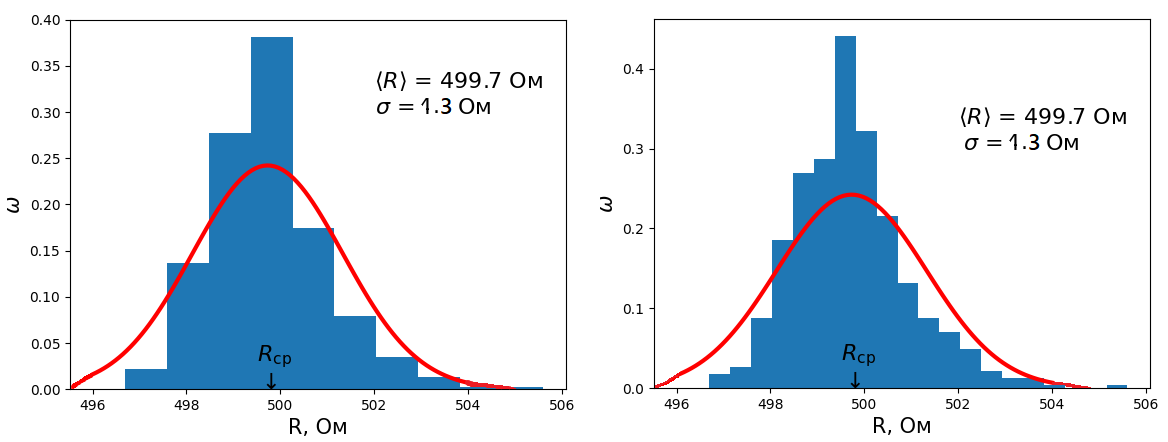
\includegraphics[width=1.05\linewidth]{all.lab.png}
     \caption{Гистограммы для $m = 10$ и $m = 20$ соответственно (работа в группе по 4 человека)}
     \label{fig:enter-label}
 \end{figure} 
 
\newpage
               \begin{flushright}
  \textbf{Таблица 1.}
  
  \textit{Результаты измерения сопротивления 270 резисторов (Ом)}
 \end{flushright}
    \begin{table}[!ht]
    \centering
    \begin{tabular}{|l|l|l|l|l|l|l|l|l|}
    \hline
        498 & 498.6 & 496.9 & 498 & 500.5 & 500.4 & 496.9 & 500.5 & 498.6 \\ \hline
        500.5 & 500.6 & 497.3 & 500.5 & 498.7 & 499.6 & 497.3 & 498.7 & 500.6 \\ \hline
        498.9 & 499.9 & 497.9 & 498.9 & 499.8 & 499.4 & 497.9 & 499.8 & 499.9 \\ \hline
        500.2 & 499.9 & 498.1 & 500.2 & 500.2 & 500.2 & 498.1 & 500.2 & 499.9 \\ \hline
        499.4 & 502.6 & 498.1 & 499.4 & 500 & 499.82 & 498.1 & 500 & 502.6 \\ \hline
        498.8 & 498.7 & 498.2 & 498.8 & 500.3 & 498.2 & 498.2 & 500.3 & 498.7 \\ \hline
        501 & 499.5 & 498.4 & 501 & 501.8 & 498.5 & 498.4 & 501.8 & 499.5 \\ \hline
        499.7 & 499.6 & 498.4 & 499.7 & 501.7 & 499.3 & 498.4 & 501.7 & 499.6 \\ \hline
        500.06 & 501.6 & 498.5 & 500.06 & 499.95 & 499.9 & 498.5 & 499.95 & 501.6 \\ \hline
        500 & 500.2 & 498.6 & 500 & 499.6 & 499.9 & 498.6 & 499.6 & 500.2 \\ \hline
        500.2 & 498.8 & 498.6 & 500.2 & 499.5 & 498.7 & 498.6 & 499.5 & 498.8 \\ \hline
        500.7 & 498.7 & 498.8 & 500.7 & 499.5 & 498.7 & 498.8 & 499.5 & 498.7 \\ \hline
        499.3 & 499.55 & 499.2 & 499.3 & 503.1 & 499 & 499.2 & 503.1 & 499.55 \\ \hline
        500.5 & 499.8 & 499.2 & 500.5 & 499.4 & 500.1 & 499.2 & 499.4 & 499.8 \\ \hline
        498.6 & 501.1 & 499.3 & 498.6 & 500.1 & 500.5 & 499.3 & 500.1 & 501.1 \\ \hline
        499.3 & 501.2 & 499.3 & 499.3 & 499.8 & 500.4 & 499.3 & 499.8 & 501.2 \\ \hline
        500.3 & 499.8 & 499.3 & 500.3 & 499.5 & 498.9 & 499.3 & 499.5 & 499.8 \\ \hline
        499.5 & 501.8 & 499.3 & 499.5 & 501.7 & 498.4 & 499.3 & 501.7 & 501.8 \\ \hline
        499.5 & 499.4 & 499.7 & 499.5 & 500.8 & 499 & 499.7 & 500.8 & 499.4 \\ \hline
        500.9 & 498.9 & 499.7 & 500.9 & 498.7 & 498.6 & 499.7 & 498.7 & 498.9 \\ \hline
        499.9 & 500.4 & 499.9 & 499.9 & 500.5 & 498.2 & 499.9 & 500.5 & 500.4 \\ \hline
        500.3 & 502.5 & 500.2 & 500.3 & 498.4 & 498.1 & 500.2 & 498.4 & 502.5 \\ \hline
        499.6 & 500.3 & 500.3 & 499.6 & 498.5 & 502.2 & 500.3 & 498.5 & 500.3 \\ \hline
        502.6 & 499.2 & 500.5 & 502.6 & 498.3 & 501.1 & 500.5 & 498.3 & 499.2 \\ \hline
        501.5 & 501.2 & 500.5 & 501.5 & 502.1 & 501.3 & 500.5 & 502.1 & 501.2 \\ \hline
        500.5 & 501.4 & 500.7 & 500.5 & 500.5 & 501.7 & 500.7 & 500.5 & 501.4 \\ \hline
        500.2 & 499.1 & 500.9 & 500.2 & 500 & 501.3 & 500.9 & 500 & 499.1 \\ \hline
        501.4 & 498.4 & 501 & 501.4 & 499.3 & 500.7 & 501 & 499.3 & 498.4 \\ \hline
        497.6 & 499.4 & 501.2 & 497.6 & 503.2 & 499.2 & 501.2 & 503.2 & 499.4 \\ \hline
        499.7 & 502.1 & 502.9 & 499.7 & 498.8 & 499.65 & 502.9 & 498.8 & 502.1 \\ \hline
    \end{tabular}
\end{table}
\newpage
    \begin{flushright}
        \textbf{Таблица 2.}
 \end{flushright}
\begin{table}[!ht]
    \centering
    \begin{tabular}{|l|l|l|l|l|l|l|l|l|l|l|}
    \hline
        $k$ & 1 & 2 & 3 & 4 & 5 & 6 & 7 & 8 & 9 & 10 \\ \hline
        $\omega \cdot 1000$ & 29 & 74 & 235 & 286 & 357 & 342 & 150 & 126 & 70 & 69 \\ \hline
        $\Delta n$ & 5 & 11 & 36 & 44 & 55 & 53 & 23 & 20 & 11 & 11 \\ \hline
    \end{tabular}
\end{table}
    \begin{flushright}
        \textbf{Таблица 3.}
 \end{flushright}
\begin{table}[!ht]
    \centering
    \begin{tabular}{|l|l|l|l|l|l|l|l|l|l|l|}
    \hline
        $k$ & 1 & 2 & 3 & 4 & 5 & 6 & 7 & 8 & 9 & 10  \\ \hline
        $\omega \cdot 1000 & 25 & 25 & 25 & 106 & 170 & 270 & 185 & 370 & 370 & 347  \\ \hline
        $\Delta n$ & 2 & 2 & 2 & 9 & 14 & 22 & 15 & 31 & 31 & 29  \\ \hline
        
    \end{tabular}
    \end{table}
        \begin{table}[!ht]
    \centering
    \begin{tabular}{|l|l|l|l|l|l|l|l|l|l|l|}
    \hline
        $k$ & 11 & 12 & 13 & 14 & 15 & 16 & 17 & 18 & 19 & 20  \\ \hline
        $\omega \cdot 1000 & 343 & 285 & 142 & 165 & 105 & 105 & 54 & 25 & 52 & 77  \\ \hline
        $\Delta n$ & 29 & 24 & 12 & 14 & 9 & 9 & 4 & 2 & 4 & 6  \\ \hline
        
    \end{tabular}
    \end{table}

   
        \section{Обсуждение результатов}
        По результатам измерений получили среднее значение сопротивления 499,9 Ом $\approx$ 500 Ом, что соответствует номиналу резистора, выяснили, какова вероятность попадания сопротивления в интервал от $\langle R\rangle - \sigma$ до $\langle R\rangle + \sigma$ (34\%) и от $\langle R\rangle - 2\sigma$ до $\langle R\rangle + 2\sigma$ (99\%), что приближенно соответствует теоретической вероятности (68\% и 95\% соответственно).

        С помощью гистограмм наглядно проиллюстрировали плотность распределения. В нашей работе количество "корзин" (или бинов) равнялось 10 и 20. В случае с $m = 20$  получили гистограмму, которая более точно описывает вероятность распределния. 

        Среднее значение сопротивления приближенно соответствует максимуму кривой нормальной распределения и бину гистограммы с наибольшей плотностью распределения, что говорит о корректности измерений.
        \section{Заключение}
        При объединении результатов измерений 4-х человек получили гистограммы, которые по величинам плотности распределения незначительно отличаются от результатов индивидуальной работы, что говорит об отсутствии грубых ошибок при замере сопротивления.

        Функция распределения Гаусса (формула (5)) приближенно ложится на гистограмму, что свидетельствует о корректности построения графиков.

        Среднее значение сопротивления, полученное экспериментальным путем ($\approx 500$ Ом), соответствует теоретическим сведениям, следовательно, при измерении отсутствовали грубые ошибки.
	\end{document}